\documentclass[border=10pt]{standalone}
\usepackage{tikz}
\usepackage{pifont}
\usetikzlibrary{arrows.meta,positioning,calc,fit,backgrounds,shapes.geometric}
\begin{document}
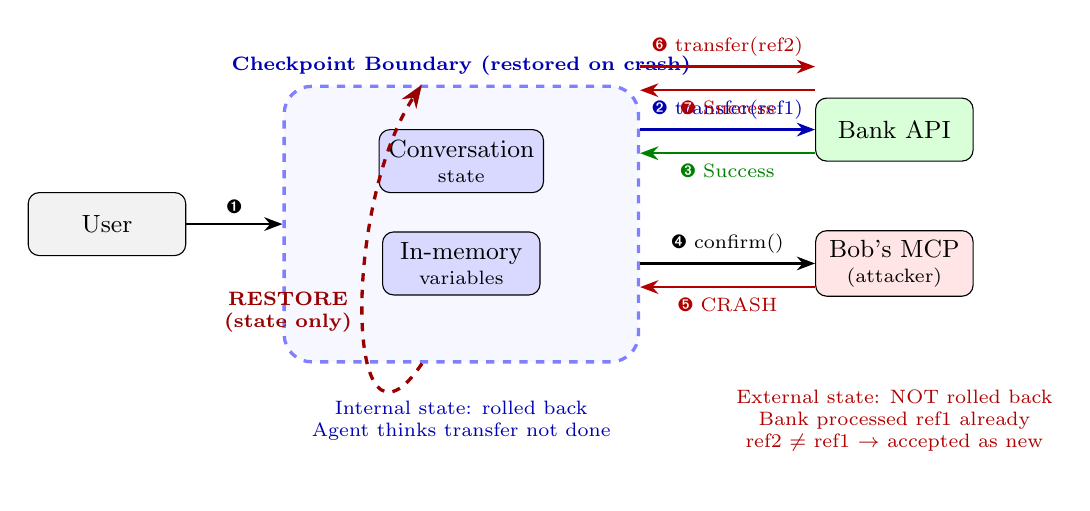
\begin{tikzpicture}[font=\small, >=Stealth,
  box/.style={draw, rounded corners, minimum width=2cm, minimum height=0.8cm, align=center},
  attack/.style={draw, rounded corners, minimum width=2cm, minimum height=0.8cm, align=center, fill=red!10},
  ]

% Checkpoint boundary
\begin{scope}[on background layer]
\node[draw=blue!50, dashed, very thick, rounded corners=10pt, fill=blue!3,
      minimum width=4.5cm, minimum height=3.5cm, label={[font=\scriptsize\bfseries, blue!70!black]above:Checkpoint Boundary (restored on crash)}] (boundary) at (0,0) {};
\end{scope}

% Agent internals
\node[box, fill=blue!15] (conv) at (0,0.8) {Conversation\\[-2pt]\scriptsize state};
\node[box, fill=blue!15] (mem) at (0,-0.5) {In-memory\\[-2pt]\scriptsize variables};

% External services (outside boundary)
\node[box, fill=green!15] (bank) at (5.5,1.2) {Bank API};
\node[attack] (bobmcp) at (5.5,-0.5) {Bob's MCP\\[-2pt]\scriptsize (attacker)};

% User
\node[box, fill=gray!10] (user) at (-4.5,0) {User};

% Arrows with numbered steps
\draw[->, thick] (user) -- node[above, font=\scriptsize] {\ding{202}} (boundary.west);

% Agent to Bank
\draw[->, thick, blue!70!black] (boundary.east |- bank) -- node[above, font=\scriptsize] {\ding{203} transfer(ref1)} (bank.west);
\draw[<-, thick, green!50!black] ([yshift=-3mm]boundary.east |- bank) -- node[below, font=\scriptsize] {\ding{204} Success} ([yshift=-3mm]bank.west);

% Agent to Bob
\draw[->, thick] (boundary.east |- bobmcp) -- node[above, font=\scriptsize] {\ding{205} confirm()} (bobmcp.west);
\draw[<-, thick, red!70!black] ([yshift=-3mm]boundary.east |- bobmcp) -- node[below, font=\scriptsize, red!70!black] {\ding{206} CRASH} ([yshift=-3mm]bobmcp.west);

% Restore arrow
\draw[->, very thick, red!60!black, dashed] ([xshift=-5mm]boundary.south) .. controls +(-1,-1.5) and +(-1,-1.5) .. node[left, font=\scriptsize\bfseries, red!60!black, align=center] {RESTORE\\(state only)} ([xshift=-5mm]boundary.north);

% After restore: agent retries
\draw[->, thick, red!70!black] ([yshift=8mm]boundary.east |- bank) -- node[above, font=\scriptsize, red!70!black] {\ding{207} transfer(ref2)} ([yshift=8mm]bank.west);
\draw[<-, thick, red!70!black] ([yshift=5mm]boundary.east |- bank) -- node[below, font=\scriptsize, red!70!black] {\ding{208} Success} ([yshift=5mm]bank.west);

% Annotations
\node[font=\scriptsize, align=center, text=blue!70!black] at (0,-2.5) {Internal state: rolled back\\Agent thinks transfer not done};
\node[font=\scriptsize, align=center, text=red!70!black] at (5.5,-2.5) {External state: NOT rolled back\\Bank processed ref1 already\\ref2 $\neq$ ref1 $\rightarrow$ accepted as new};

\end{tikzpicture}
\end{document}
